%% ---------------------------------------------------------------------------------------------------------
\section{Mechanism: how a rescue and a harm happen}\label{sec:mechanism}

\paragraph{Question} Which steps of the chain observation $\to$ memory $\to$ decision $\to$ move $\to$ hand-back produce rescues, and where does harm enter? This section is descriptive and uses development records (driver 550.120); the cases were selected as stated and are not a random sample.

\paragraph{Rescue} In the typical rescue (Fig.~\ref{fig:problem}b; the first seed-1 rescue in scene order) the policy has carried the cube to a position beside the target and queued an open command there. V2 discards that command, moves the gripper towards the estimated target position, and hands back; the re-planned policy opens the gripper a few steps later (median 2--3 steps after the move in all stages) over the target, and the cube is placed.

\begin{figure}[!htbp]
\centering
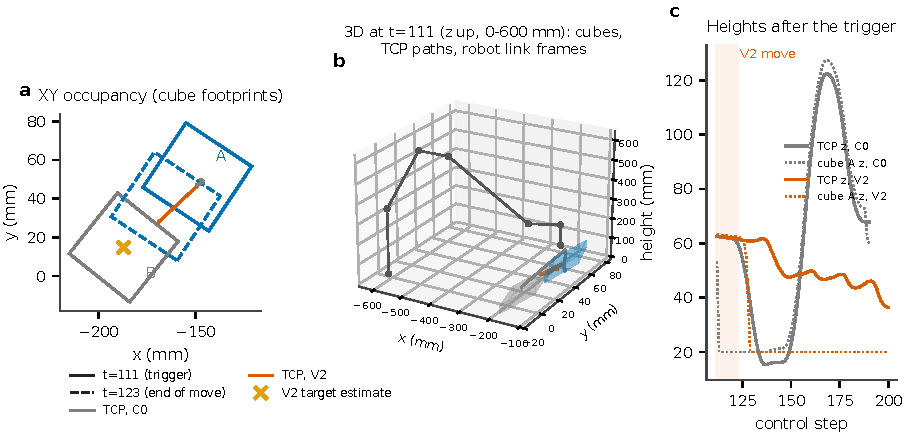
\includegraphics[width=\linewidth]{Fig05_spatial_51157.pdf}
\caption{The development harm case 51157 (policy seed 1; the only V2 harm for this policy in development). (a) Footprints of the held cube A (blue) and target cube B (grey) at the trigger (solid) and at the end of the V2 move (dashed), the TCP paths of C0 and V2 and the V2 target estimate, from the logged poses. (b) Three-dimensional view at the trigger: cube boxes from the logged poses, TCP paths of C0 (grey) and V2 (orange), and the robot link frames (origins, not collision meshes). (c) Heights of the TCP and of cube A after the trigger; the shaded band is the V2 move.}\label{fig:spatial}
\end{figure}

\paragraph{Harm} In scene 51157, the single development harm of V2 for policy seed 1, V2 did what it was designed to do. At the trigger the held cube was 54.6\,mm from the target centre; the V2 estimate was 54.7\,mm (error 0.15\,mm), within its 9\,mm reading bound. V2 moved for the full 12 steps; the TCP moved 24.3\,mm, and the true offset fell to 30.4\,mm (Fig.~\ref{fig:spatial}a). The move followed its commanded direction (cosine above 0.999 at every step, so this move passed Check 4) but not its commanded length: each 5\,mm command produced about 2\,mm of TCP displacement (Fig.~\ref{fig:control}a,b). Three steps after the hand-back the re-planned policy opened the gripper with the cube still beside the target; the cube fell to the table and the policy did not regrasp it before the horizon (Fig.~\ref{fig:spatial}c). Without V2 the policy also dropped the cube beside the target, but it regrasped it and completed the stack at step 190, 10 steps before the horizon; the 12 steps spent on the move exceed that margin. The record is consistent with two contributing factors, an incomplete correction and the time budget, and it does not separate them.

\paragraph{Offsets larger than one move} Acting on an offset that one move cannot remove is a weakness of the design. Among acted scenes with an estimated offset above 40\,mm there were 3 in development (1 rescue and 1 harm, the latter being 51157), none in calibration, and 8 in the Final Test (6 rescues and 1 harm, the only harm of the test).

\begin{figure}[!htbp]
\centering
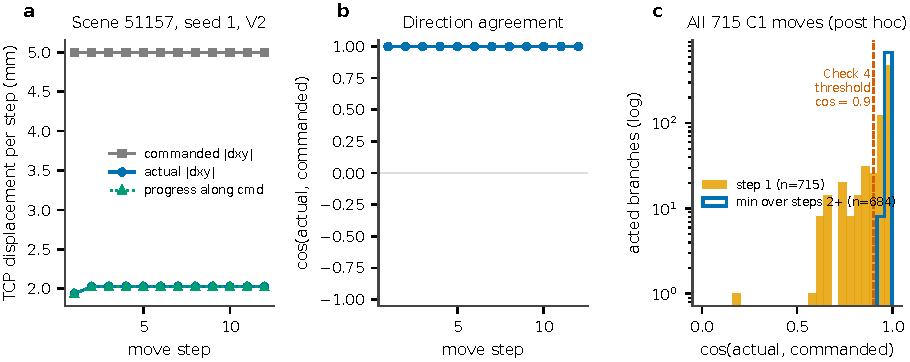
\includegraphics[width=\linewidth]{Fig06_control_check4.pdf}
\caption{Commanded versus executed motion. (a,b) Scene 51157, V2: commanded and executed horizontal TCP displacement per move step and their direction cosine. (c) All 715 acted development branches of all arms (post hoc): cosine between executed and commanded horizontal step, for the first step and for the minimum over steps 2 onwards (log scale). 110 branches fall below the pre-declared 0.9 threshold at the first step and none at later steps; the cause of the first-step deviation is not established.}\label{fig:control}
\end{figure}

\paragraph{The pre-declared motion check} Check 4 required, for every move step, a cosine of at least 0.9 between the executed and the commanded horizontal TCP step, and an executed step length of at least 0.2\,mm. It failed in 9 of 41 V2 moves for policy seed 1 and 5 of 39 for seed 2; we keep the official FAIL. In all 14 failures only the first step failed, and only on direction (cosine 0.63--0.88); the later steps of the same moves had cosine 0.934--0.999. Across all arms, 110 of 715 moves failed, all at the first step; a post hoc check of steps 2 onwards passed in all 715 (Fig.~\ref{fig:control}c). The failing V2 moves had a lower cosine between the first command and the TCP motion just before the trigger (median $-0.57$ against $0.66$ for passing moves), which is consistent with the arm still carrying the policy's previous motion; we did not log controller internals, so this association is not an established cause.

\paragraph{Missed rescues} The oracle rescued 15 and 21 development scenes; V2 rescued 14 and 16. Of the oracle rescues, V2 missed 1 (policy seed 1) and 5 (policy seed 2), all by abstaining: side-contact risk (2), held cube too low (2), no target estimate (1), and aligned within the reading bound (1). Supplementary Table~S3 lists the decisions of every stage.

\paragraph{Limits} The mechanism is descriptive, read from development records on driver 550.120, and is not a causal decomposition. Scene 51157 is one case; its C0 branch has a different outcome on the calibration host, so the case describes the development configuration rather than the certified one.
